\documentclass[aspectratio=169]{beamer}
\usetheme{Madrid}
\usecolortheme{seahorse}
\usepackage{graphicx}
\usepackage{booktabs}
\usepackage{xcolor}

\setbeamertemplate{navigation symbols}{}
\setbeamertemplate{footline}[frame number]

\title{Geminio: Language-Guided Gradient Inversion Attacks in Federated Learning}
\subtitle{Phase 1 \& 2 Progress Report}
\author{Dan Zimmerman}
\institute{Advisor: Dr. Ahmed Imteaj}
\date{\today}

\begin{document}

% --- Slide 1: Title ---
\begin{frame}
\titlepage
\end{frame}

% --- Slide 2: Background & Method ---
\begin{frame}{Background \& Attack Mechanism}
\begin{columns}[T]
\begin{column}{0.55\textwidth}
\textbf{Federated Learning (FL) Threat Model:}
\begin{itemize}
    \item Clients train locally on \textbf{private data} and share only gradients
    \item Malicious server performs \textbf{Gradient Inversion Attack (GIA)} to reconstruct private images from shared gradients
    \item \textbf{Problem:} Existing GIAs fail at large batch sizes ($\geq$64)
\end{itemize}

\vspace{0.3cm}
\textbf{Geminio's Key Contribution:}
\begin{itemize}
    \item Uses \textbf{CLIP} (Vision-Language Model) to enable \textbf{natural language queries} targeting specific private data
    \item \textbf{Reshapes the model's loss surface} so query-matching images produce dominant gradients
    \item Enables targeted reconstruction even from \textbf{128-sample batches}
\end{itemize}
\end{column}
\begin{column}{0.42\textwidth}
\centering
\includegraphics[width=\textwidth]{../assets/intro-git.png}

\vspace{0.3cm}
{\footnotesize \textit{Jiao et al., ``Geminio,'' ICCV 2025}}
\end{column}
\end{columns}
\end{frame}

% --- Slide 3: Results ---
\begin{frame}{Experimental Results --- ImageNet (128 Private Samples)}
\begin{columns}[T]
\begin{column}{0.62\textwidth}
\centering
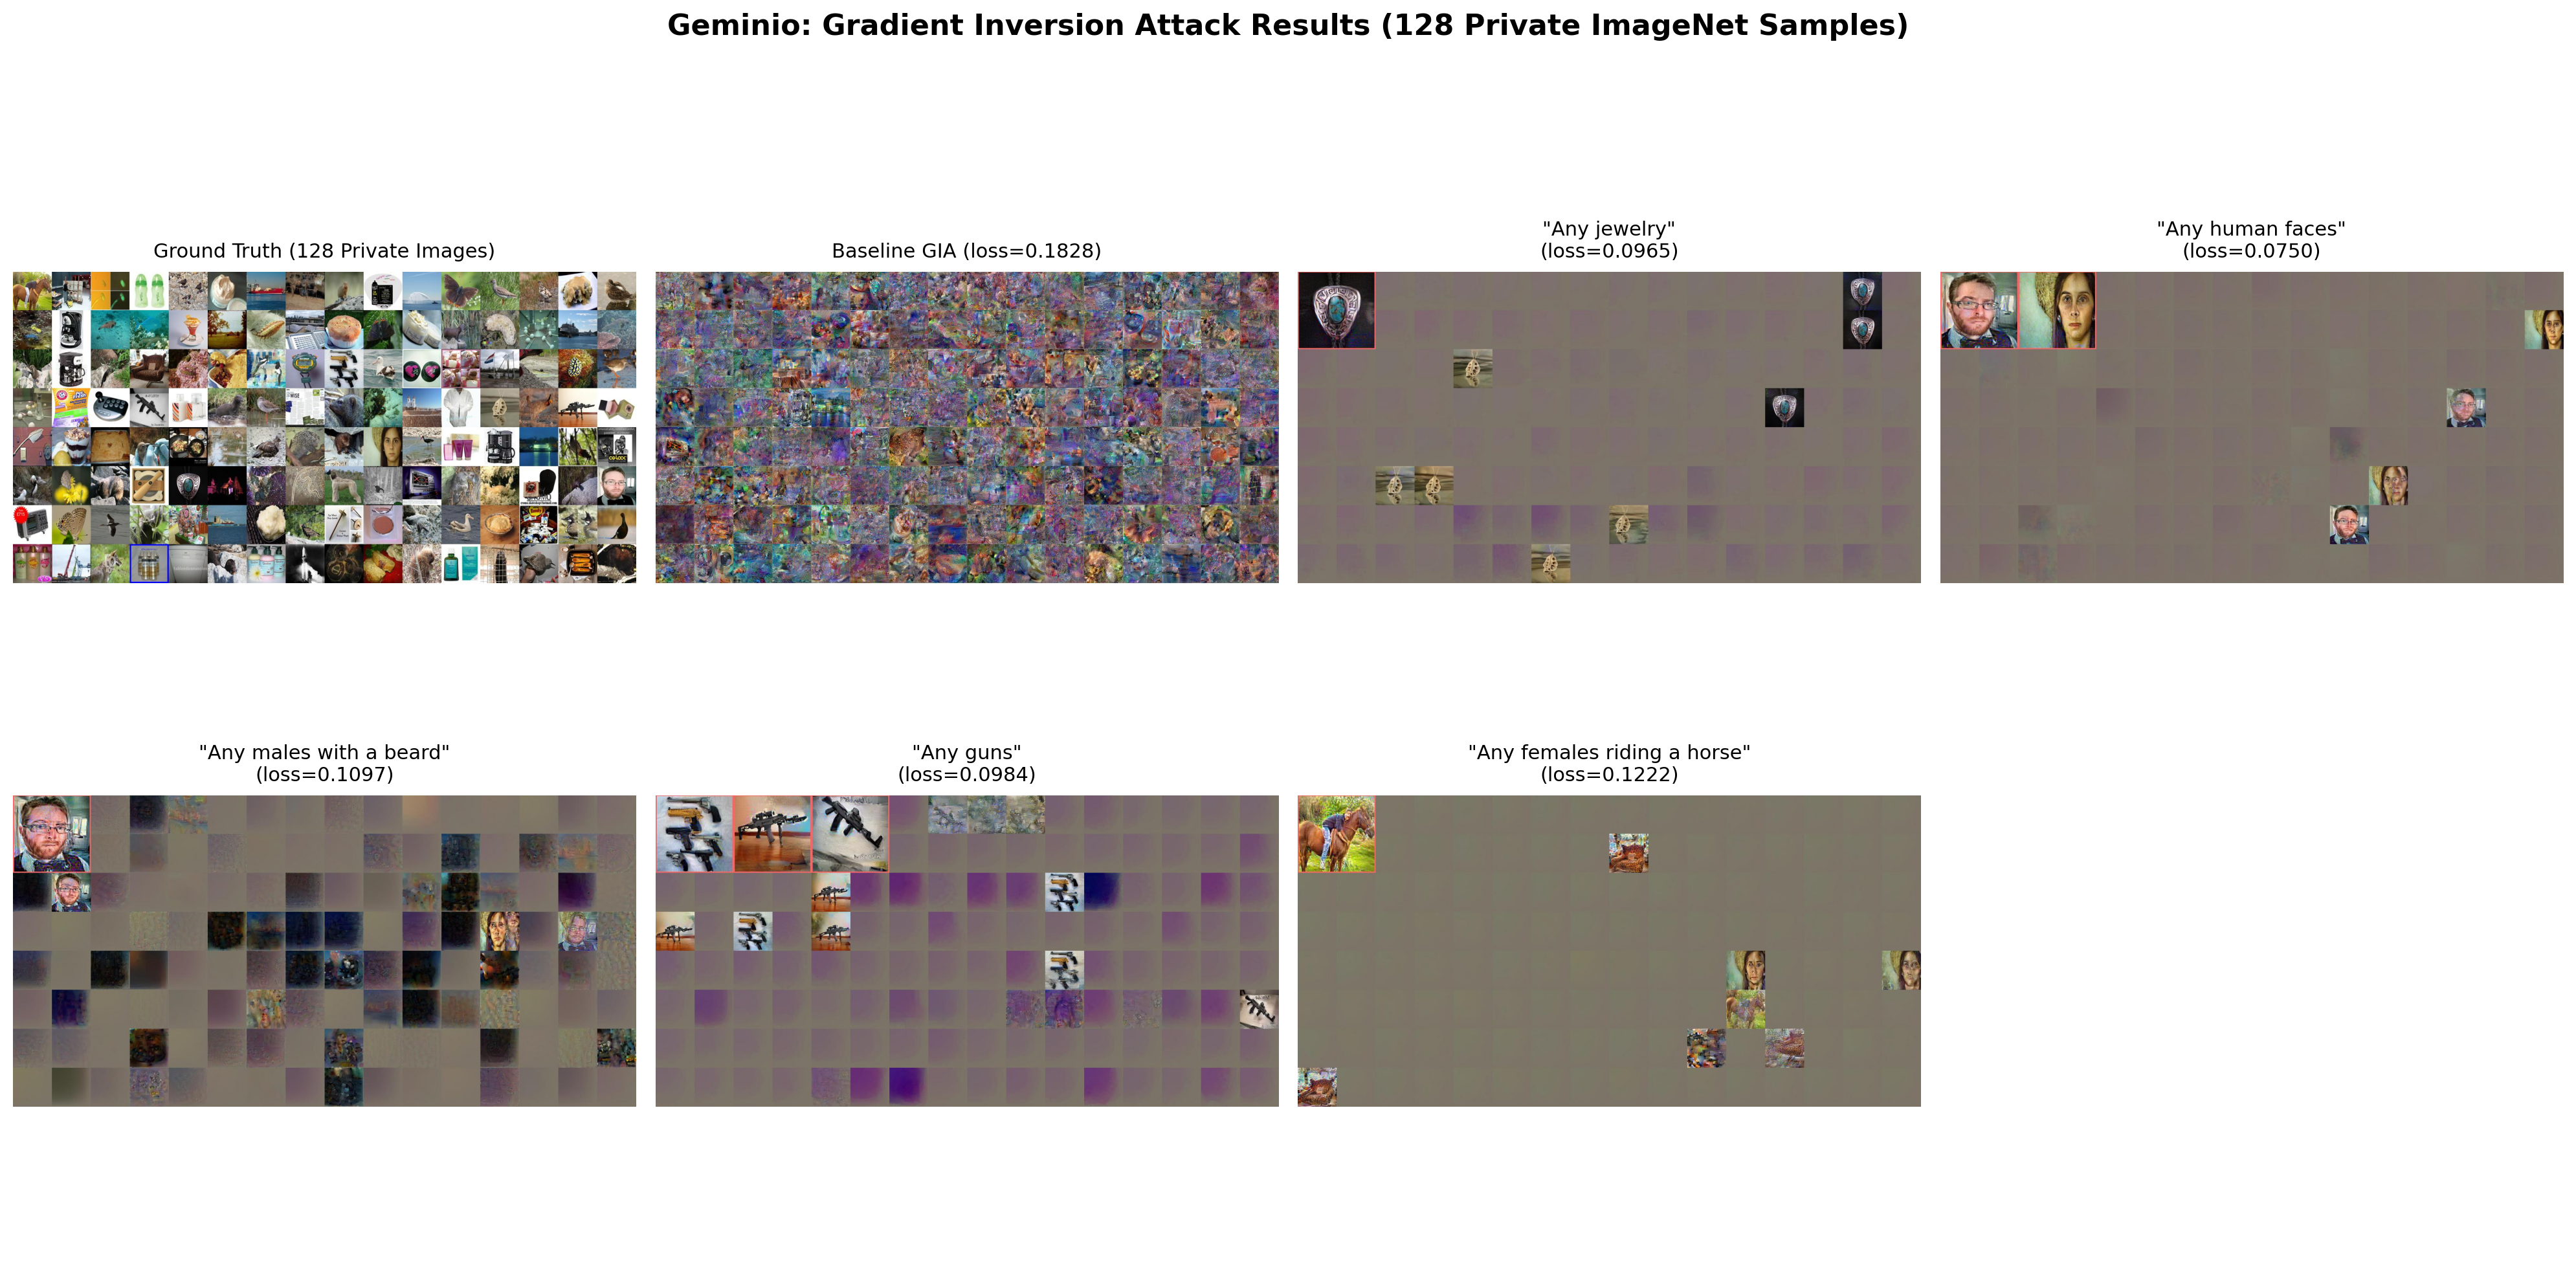
\includegraphics[width=\textwidth]{figures/full_overview.png}
\end{column}
\begin{column}{0.35\textwidth}
\textbf{Reconstruction Loss:}
\vspace{0.2cm}

\begin{tabular}{lc}
\toprule
\textbf{Method} & \textbf{Loss} \\
\midrule
Baseline GIA & 0.1828 \\
\midrule
\multicolumn{2}{l}{\textit{Geminio (ours):}} \\
~~Jewelry & 0.0965 \\
~~Human faces & \textbf{0.0750} \\
~~Bearded males & 0.1097 \\
~~Guns & 0.0984 \\
~~Female on horse & 0.1222 \\
\bottomrule
\end{tabular}

\vspace{0.3cm}
{\footnotesize
\textbf{Key findings:}
\begin{itemize}
    \item Baseline: all 128 images unrecognizable
    \item Geminio: query-matched images clearly reconstructed
    \item Non-matched images suppressed (gray)
    \item Best: ``human faces'' (47\% lower loss vs baseline)
\end{itemize}
}
\end{column}
\end{columns}
\end{frame}

% --- Slide 4: Next Steps ---
\begin{frame}{Next Steps --- Healthcare Application}
\textbf{Completed (Phases 1--2):}
\begin{itemize}
    \item[\checkmark] Paper review and understanding of attack mechanism
    \item[\checkmark] Full pipeline reproduced on ImageNet: VLM embeddings $\rightarrow$ malicious model training $\rightarrow$ gradient inversion attacks
    \item[\checkmark] Debugged and documented implementation issues (dependency conflicts, missing configs, data path issues)
\end{itemize}

\vspace{0.4cm}
\textbf{Phase 3 --- Healthcare Dataset Application:}
\begin{itemize}
    \item Apply Geminio to \textbf{medical images} (MRI, X-ray, patient records)
    \item Demonstrate whether sensitive patient data can be exposed despite FL privacy guarantees
    \item \textbf{Adaptation needed:} Replace CLIP with medical VLM (e.g., BiomedCLIP) for better medical image--text alignment
    \item Queries would target medical conditions: e.g., \textit{``Any chest X-ray showing pneumonia''}
\end{itemize}

\vspace{0.4cm}
\textbf{Future Directions:}
\begin{itemize}
    \item Propose \textbf{defense mechanisms} (not covered in original paper)
    \item Explore applicability to \textbf{DoD/mission-critical} settings
\end{itemize}
\end{frame}

\end{document}
